\subsection{Introduction}

Four experiment caverns are foreseen at FCC. 
During the FCC-ee operation, all these caverns will house general-purpose detectors, 
with various degrees of specialisation, aimed at exploiting the full physics potential of this collider.
During the \mbox{FCC-hh} operation, a layout similar to the present LHC is foreseen: 
two caverns will house general-purpose detectors that cover the entirety of the proton-proton physics programme, 
similar to ATLAS and CMS, and the other two will house detectors more specialised to dedicated physics topics, 
on the model of ALICE and LHCb. 
It would be highly inefficient, impractical, and costly to modify the caverns at the end of the FCC-ee phase.
A common cavern infrastructure that will serve equally well FCC-ee and FCC-hh must therefore be designed ahead of time.

Most aspects of the FCC experimental cavern infrastructure are defined by requirements for the FCC-hh detectors, 
given their much larger size, the extreme radiation environment and related shielding, as well as larger magnetic stray fields. 
A reference detector, conceived as a general-purpose detector able to fully exploit the physics potential of FCC-hh, 
was studied in detail in Ref.~\cite{Mangano:2022ukr}. 
A cavern size of L66\,m $\times$ W35\,m $\times$ H35\,m with a shaft diameter of 18\,m 
is deemed sufficient to install and house such a detector. 
The cross section of this cavern is very similar to that of the ATLAS experiment. 
Two caverns of this size and two smaller caverns for the specialised experiments have therefore been assumed 
to define the corresponding civil-engineering operations and costs.

To evaluate their size, the two smaller caverns were assumed to house 
a detector specialised in \PB-physics, on the one hand, and 
a detector specialised in heavy-ion physics, on the other. 
Preliminary studies~\cite{Chobanova:2020vmx,Prouvetalk} have shown that 
a detector with transverse and longitudinal sizes not significantly larger than the dimensions of LHCb 
(10\,m and 20\,m, respectively) 
would have the same acceptance and resolutions as LHCb, in spite of the much larger energies. 
A more compact design, 
inspired from that of the BTeV detector~\cite{Kulyavtsev:1999tcg},
would allow a two-arm spectrometer to be built in the same spatial envelope. 
Similarly, a heavy-ion experiment would need to be more granular and have better performance, 
but its overall size would not have to be different from that of ALICE
(the ALICE cavern dimensions are L53.5\,m $\times$ W15.5\,m $\times$ H22.7\,m).

A transverse cavern size similar to that of the CMS experiment would therefore be sufficient for both specialised detectors, 
leading to a L66\,m $\times$ W25\,m $\times$ H24.5\,m cavern and a shaft diameter of 15\,m for those two caverns. 
Such four caverns will definitely be more than adequate to house the FCC-ee detectors, 
which have typical diameters and lengths of 12--14\,m. 
The possibility of detector opening for maintenance in these caverns, especially the smaller ones, 
still need to be fully understood and ascertained.

In the following sections, 
the specifications and the layout of the FCC-hh reference detector are summarised, 
and more details on the cavern layout are given.

\subsection{The FCC-hh reference detector}

The FCC-hh parameters allow the direct exploration of particles with mass up to 
around 40--50\,TeV~\cite{Golling:2016gvc}, 
approximately an order of magnitude over the LHC sensitivity to heavy resonant states. 
During its lifetime, the FCC-hh is also expected to produce trillions of top quarks and tens of billions of Higgs bosons, 
allowing for rich SM precision measurement campaign~\cite{Contino:2016spe,fcc-phys-cdr} 
and rare-decay study programme~\cite{dEnterria:2023wjq}. 
Most importantly, FCC-hh is the only machine under study today that can provide 
a few per-cent level measurement of the Higgs boson self-coupling~\cite{Contino:2016spe,Mangano:2020sao}. 

An experimental apparatus that operates at FCC-hh must, hence, 
perform optimally on two main fronts (see Ref.~\cite{Mangano:2022ukr} for a thorough discussion). 
Firstly, physics at the EW and Higgs boson scale will produce objects in the detector with momenta in the \pt range 20--100\,GeV; 
the LHC detectors were built to produce an optimal response in such an energy range. 
Secondly, a new regime, at the energy frontier, 
will be characterised by the energy scale of decay products originating from highly boosted SM particles 
and heavy resonances (potentially with mass as high as 50\,TeV). 
An FCC-hh detector must therefore be capable of reconstructing leptons, jets, top quarks, 
and Higgs and \PW/\PZ bosons with momenta as large as $\pt = 20$\,TeV. 
In short, the detector must provide accurate measurements in the full energy range between tens of~GeV and tens of~TeV.

\begin{figure}[ht]
\centering
  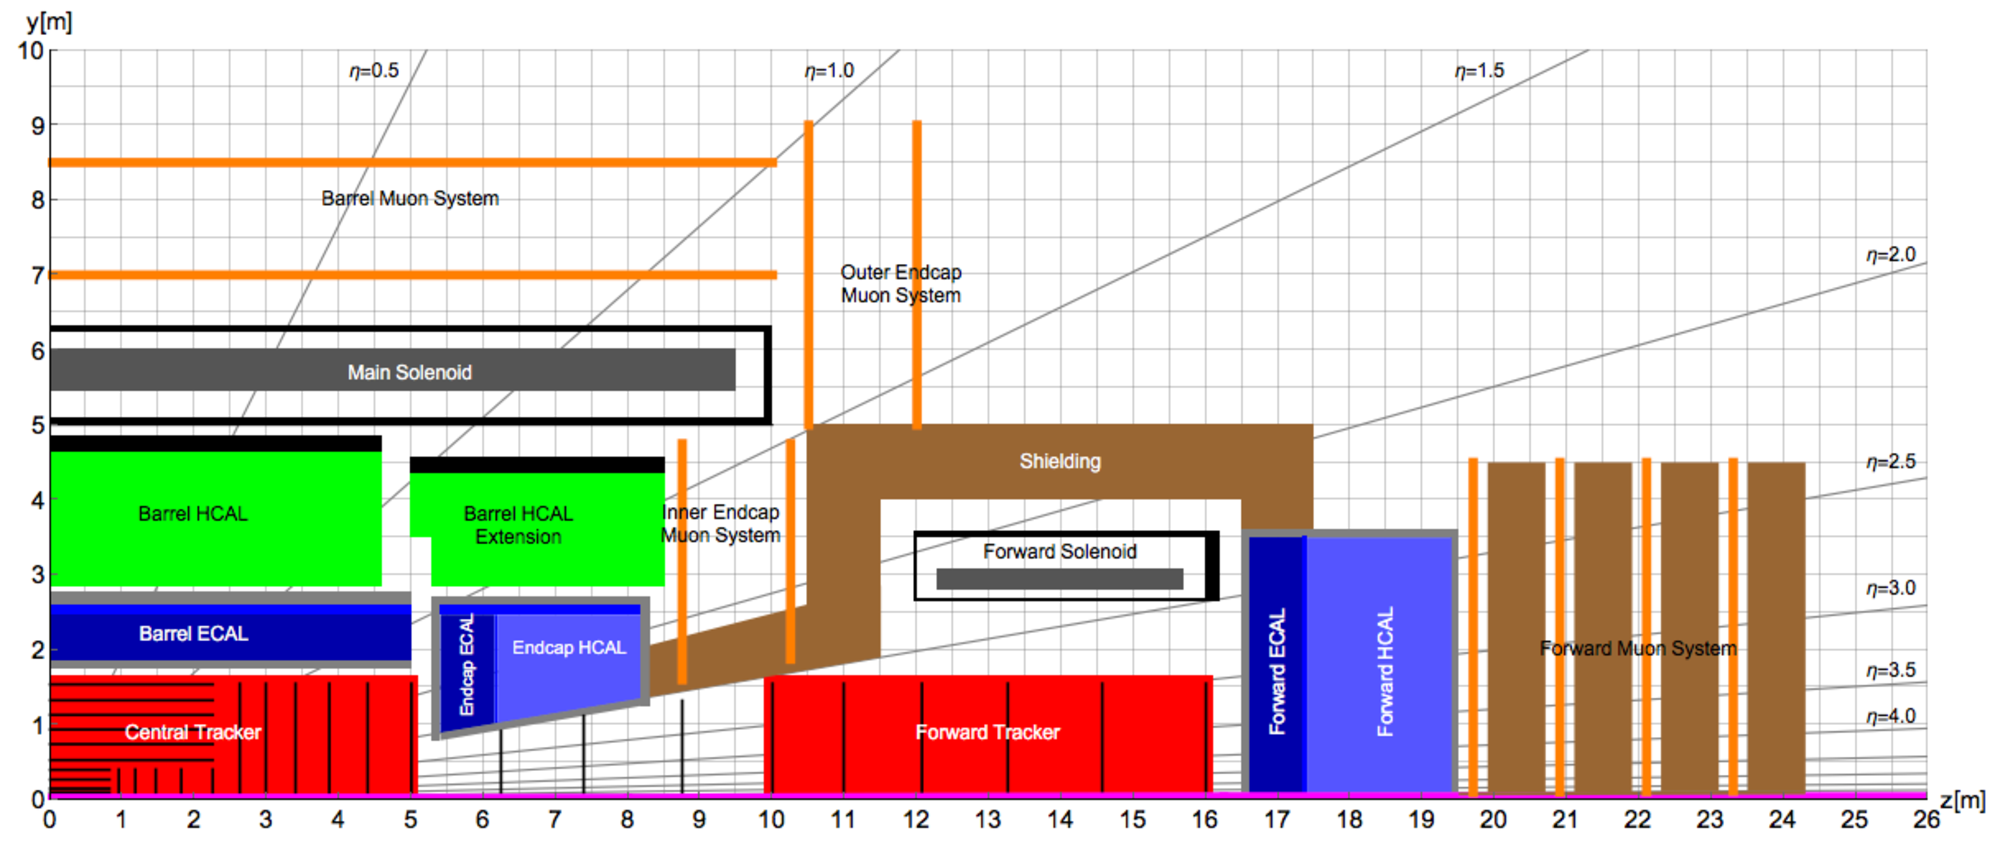
\includegraphics[width=0.85\textwidth]{Caverns/Figs/detector_2D.pdf}
  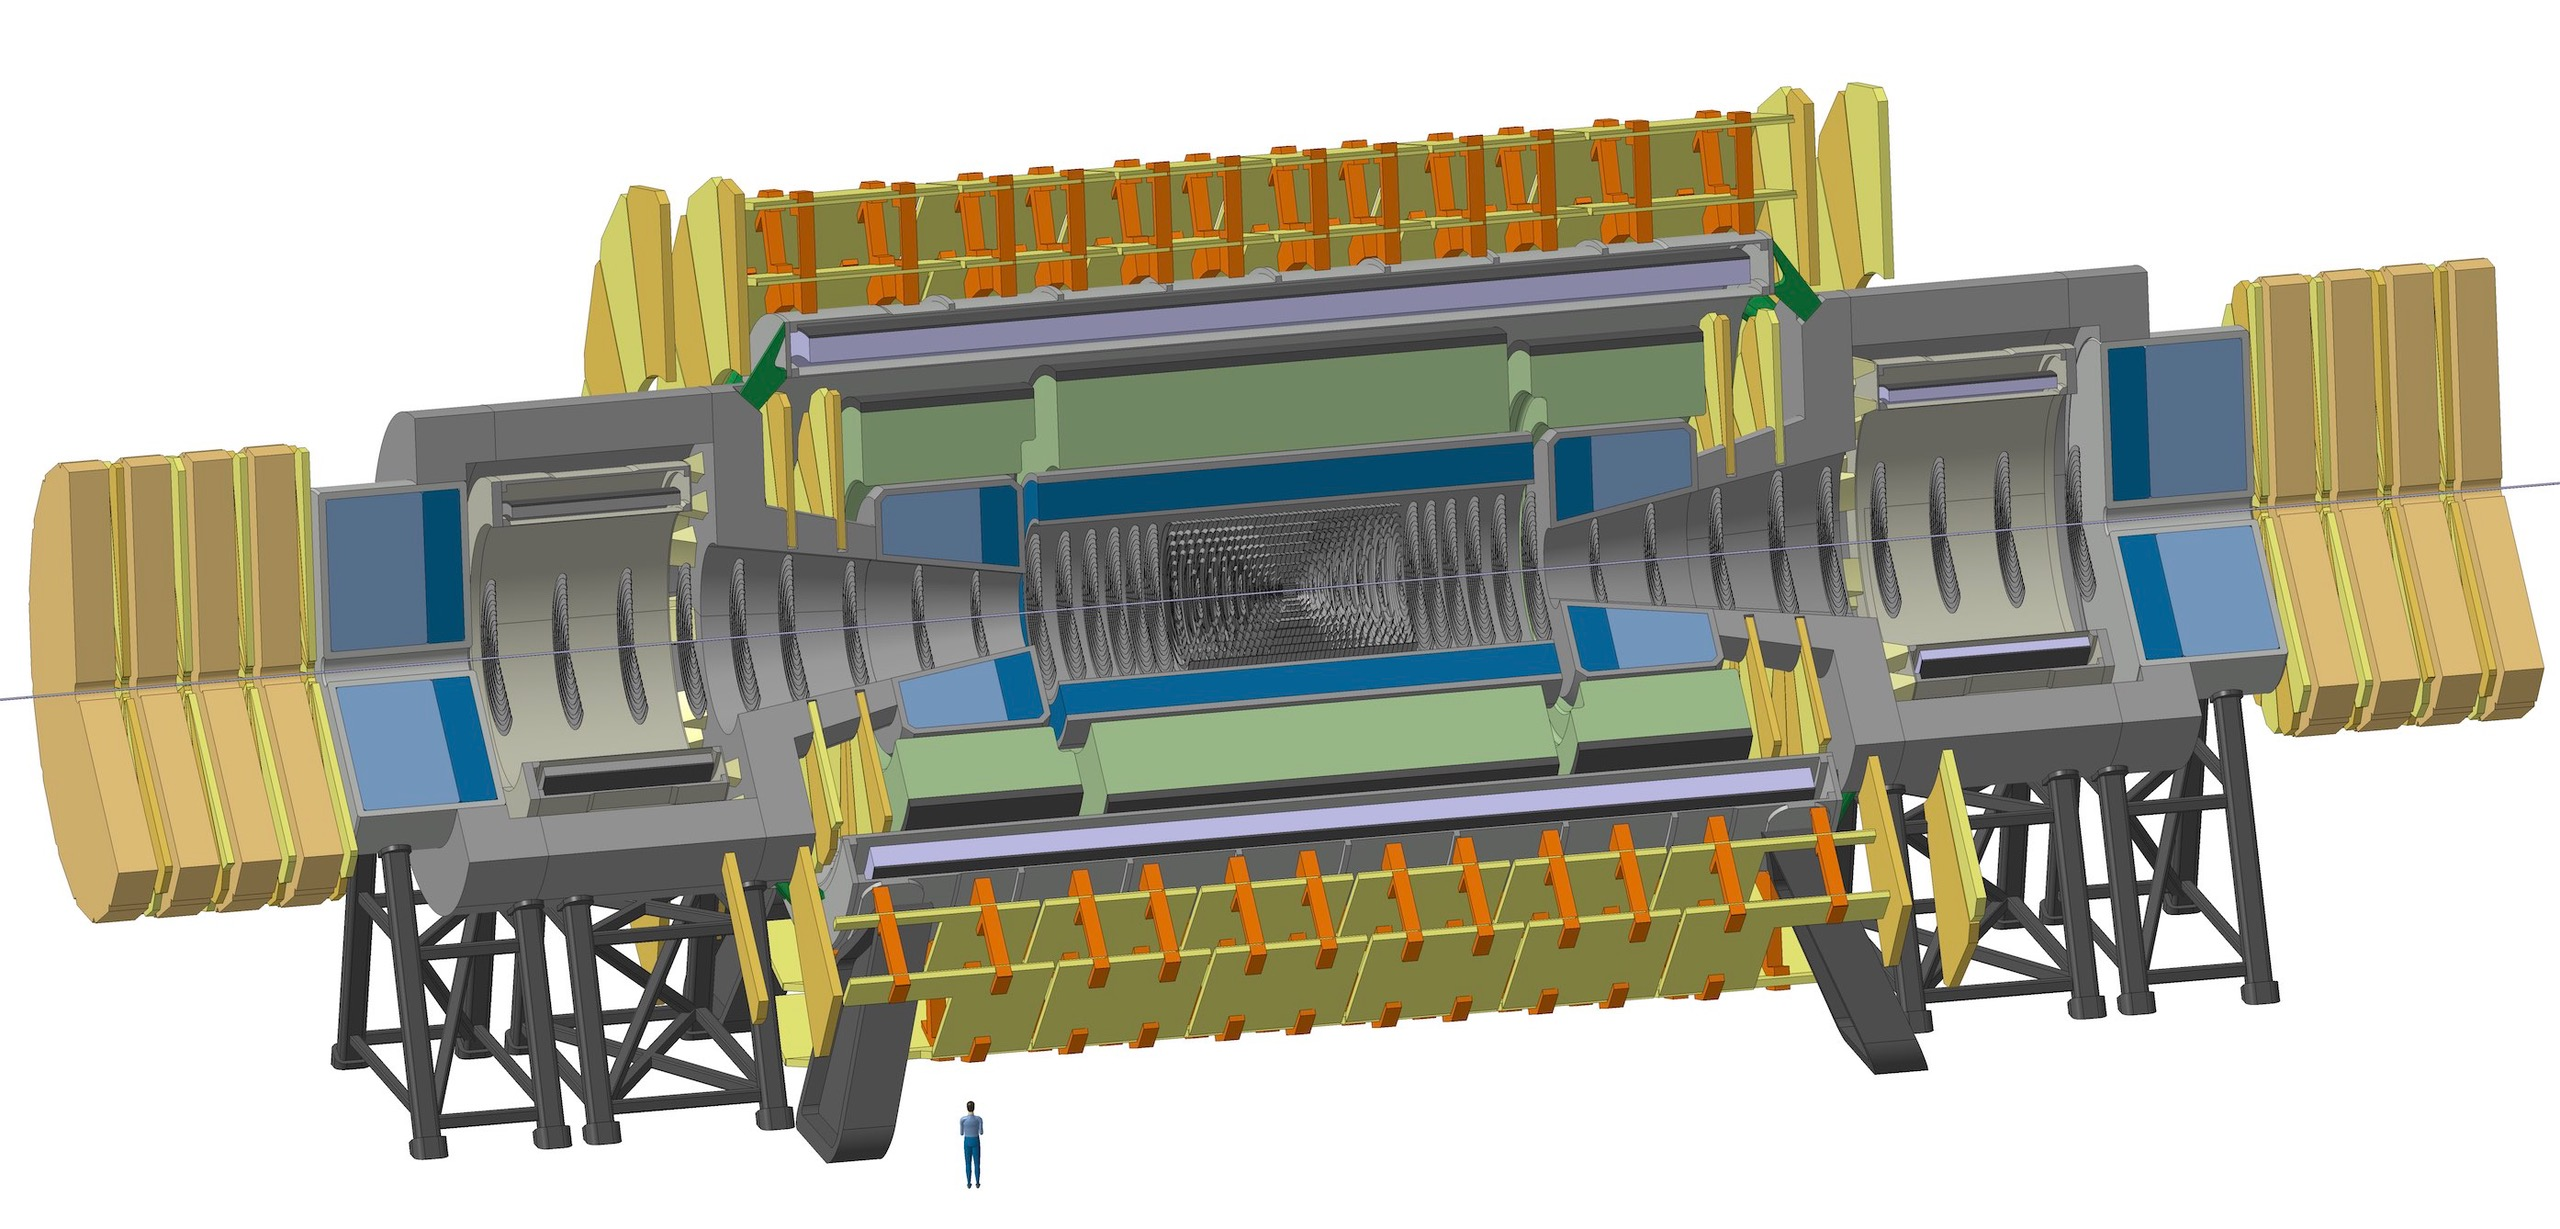
\includegraphics[width=0.85\textwidth]{Caverns/Figs/fullFCChhDet.jpeg}
  \caption{Schematic of the FCC-hh reference detector.}
  \label{FCChh-layout}
\end{figure}

Figure~\ref{FCChh-layout} shows the layout of the FCC-hh reference detector. 
This detector concept does not represent the final design, but rather a concrete example that suits the performance and physics requirements, 
and allows the identification of areas where dedicated further R\&D efforts are needed. 
The detector has a diameter of 20\,m and a length of 50\,m, comparable to the dimensions of the ATLAS detector but much heavier. 
The central detector, with a pseudorapidity coverage of $|\eta| < 2.5$, 
houses the tracking, electromagnetic calorimetry, and hadron calorimetry, inside a 4\,T solenoid with a free bore diameter of 10\,m. 
In order to reach the required performance over the $2.5 < |\eta| < 6$ pseudorapidity range, 
the forward parts of the detector are displaced along the beam axis by 10\,m from the interaction point. 
Two forward magnet coils with an inner bore of 5\,m provide the required bending power. 
These forward magnets are also solenoids with 4\,T field, 
providing a total solenoid volume of 32\,m length for high precision momentum spectroscopy up to $|\eta| \approx 4$ 
and tracking up to $|\eta| \approx 6$. 
As an option, replacing the forward solenoids with two forward dipoles is also being considered. 
The tracker cavity has a radius of 1.7\,m with the outermost layer at around 1.6\,m from the beamline in the central and forward regions, 
providing the full spectrometer arm up to $|\eta| = 3$. 
The electromagnetic calorimeter (ECAL) has a thickness of around 30 radiation lengths ($X_{0}$). 
The overall calorimeter thickness, including the hadron calorimeter (HCAL), 
exceeds 10.5 nuclear interaction lengths ($\lambda$), 
ensuring 98\,\% containment of high energy hadron showers and limiting punch-through to the muon system. 
The ECAL is based on liquid argon (LAr) given its intrinsic radiation hardness. 
The barrel HCAL is a scintillating tile calorimeter with steel and lead absorbers 
that uses wavelength shifting (WLS) fibres and silicon photomultipliers (SiPMs) for the readout. 
It is divided into a `central barrel' and two `extended barrels'. 
The HCALs for the endcap and forward regions are also based on LAr. 
The requirement of calorimetry acceptance up to $|\eta| \approx 6$ translates into 
an inner active radius of only 8\,cm at a $z$-distance of 16.6\,m from the IP. 
The transverse and longitudinal segmentation of both the electromagnetic and hadronic calorimeters 
is $\sim$\,4 times finer than the present ATLAS calorimeters.

The muon system is placed outside the magnet coils. 
The barrel muon system provides muon identification, stand-alone muon spectroscopy by measurement of the angle of the muon track, 
as well as precision muon spectroscopy by combining the tracker measurement with the measured space points in the muon chambers. 
The forward muon system can only provide spectroscopy if forward dipoles are used. 

The reference detector does not assume a magnet yoke, i.e., there is no shielding of the magnetic field.  
Figure~\ref{bfield} shows the magnetic stray field as a function of radial distance from the beamline. 
The stray field still amounts to 100\,mT at the cavern wall ($R=17.5$\,m), 
which has to be considered for the implementation of access structures and services. 
The 5\,mT level is achieved at a distance of 55\,m from the beamline, still outside of the service cavern. 
Clearly, it would be more convenient to have a shield for the magnetic field, 
but to arrive at a level of 5\,mT at the cavern wall, which was the specification for CMS, 
an iron yoke of 4\,m thickness would be required, weighing a total of 52\,kt. 

\begin{figure}[ht]
\centering
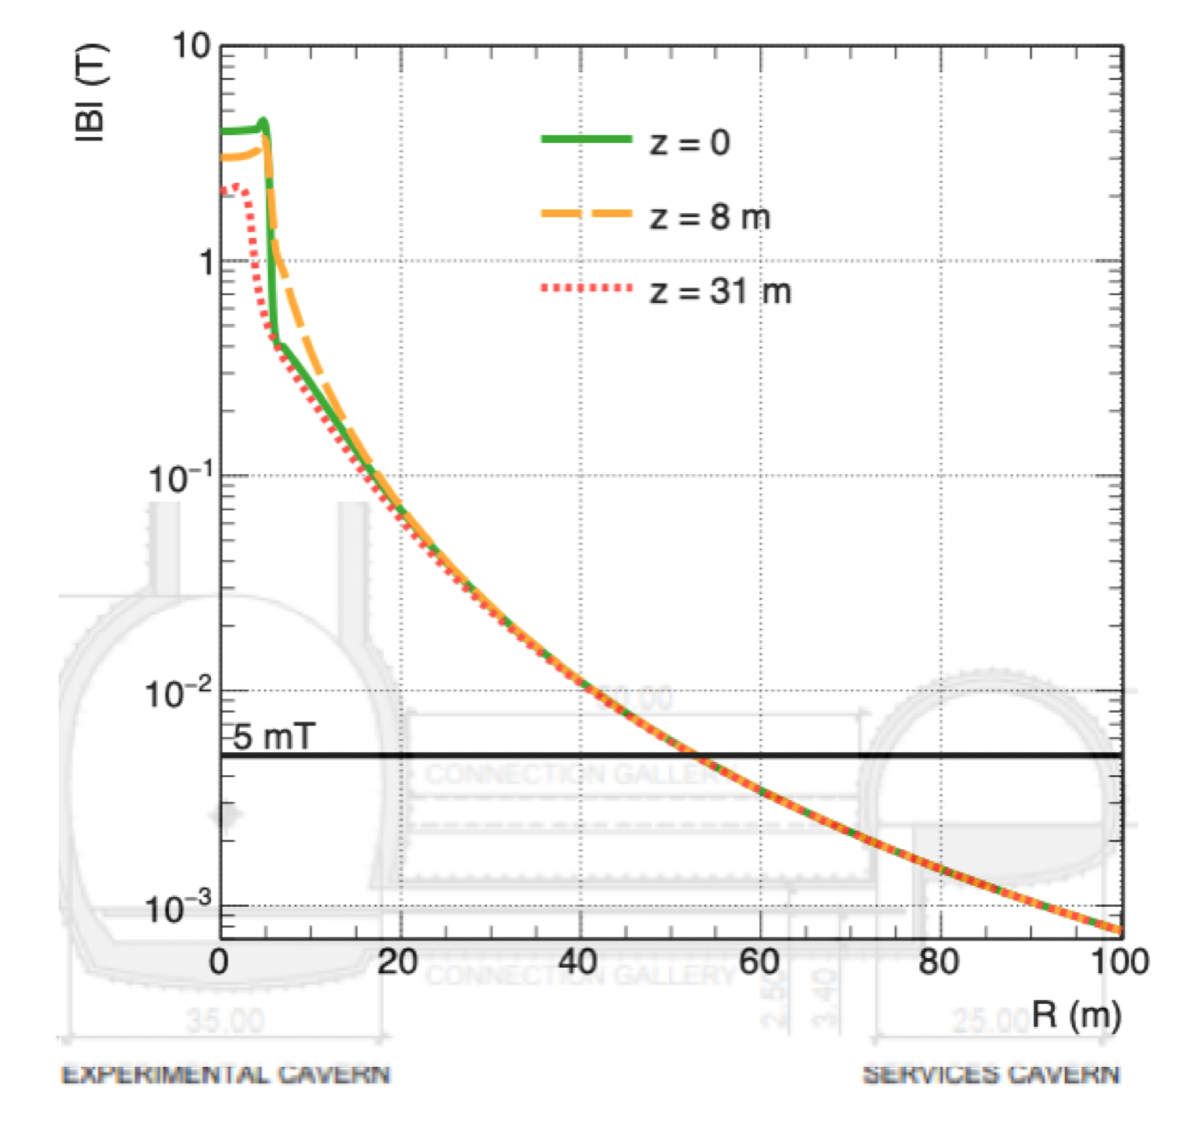
\includegraphics[width=0.6\textwidth]{Caverns/Figs/bfield_2.png}
\caption{Radial magnetic field for the FCC-hh reference detector, without magnet yoke. 
The stray field is around 100\,mT at the cavern wall, 
while in the service cavern (50\,m from the experimental cavern wall), it amounts to less than 3\,mT.}
\label{bfield}
\end{figure}

As can be seen in Fig.~\ref{FCChh-layout}, 
embedding the muon system inside a yoke of 4\,m radial thickness would lead to a total detector radius of around 11\,m, 
similar to the ATLAS detector.  
Such a yoke is probably excessive in terms of cost and construction. 
With the radial extent of around 10\,m for the \mbox{FCC-hh} reference detector, a cavern cross section of 35\,m $\times$ 35\,m is appropriate. 
If needed, such a cavern could even house the magnet yoke.  
For illustration, 
Fig.~\ref{large_cavern} shows an FCC-ee detector and the \mbox{FCC-hh} reference detector in this large cavern, while
Fig.~\ref{small_cavern} shows an FCC-ee detector and a specialised \mbox{FCC-hh} detector of 14 m-diameter, 
similar to CMS, in the smaller caverns.

\begin{figure}[t]
\centering
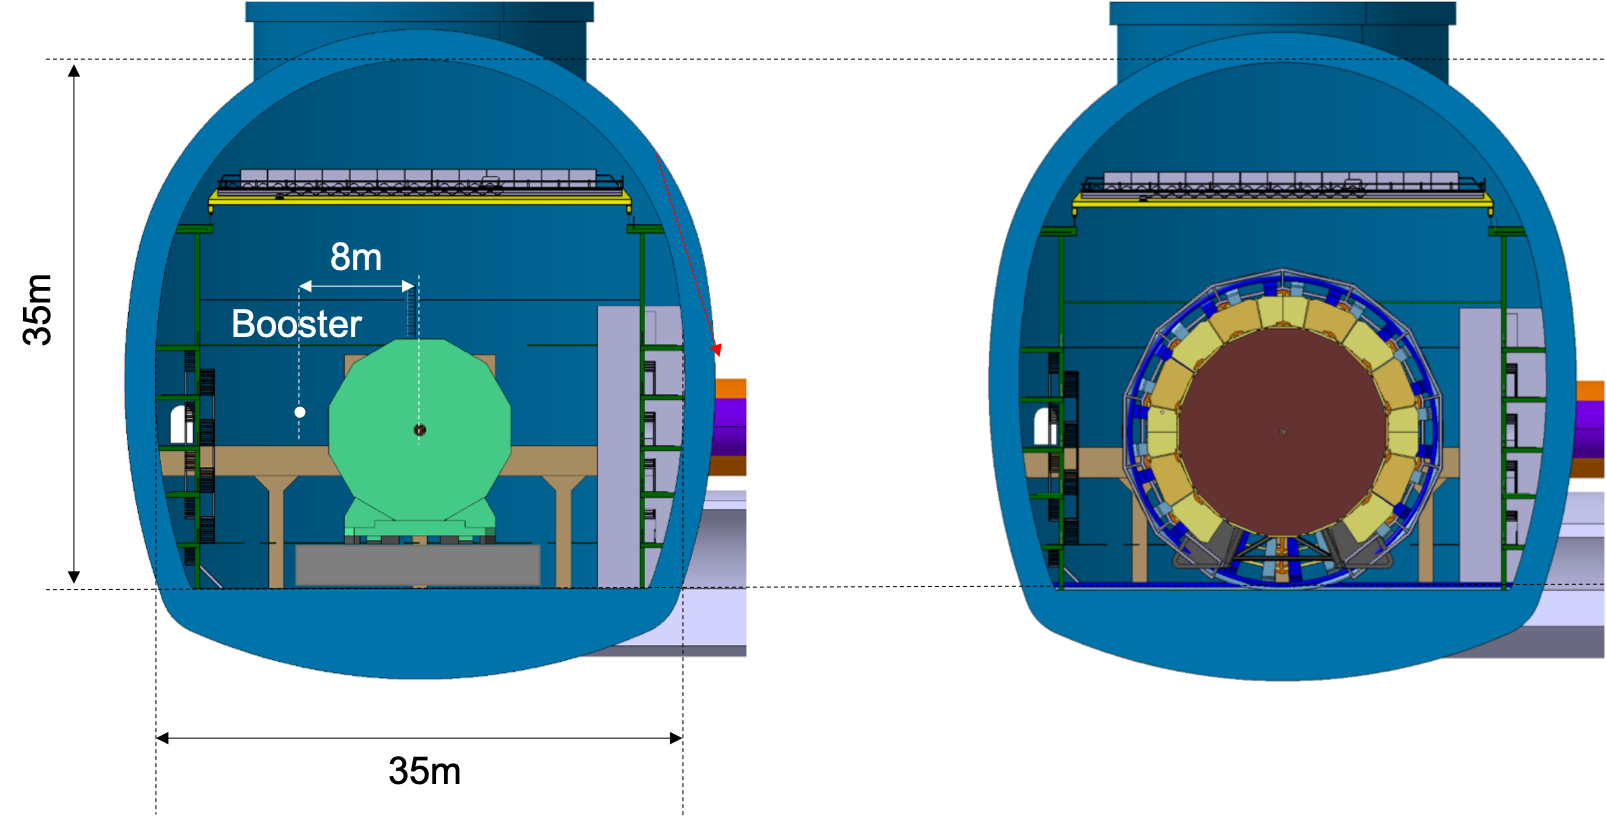
\includegraphics[width=0.9\textwidth]{Caverns/Figs/ee_hh_detector_cavern.png}
\caption{An FCC-ee detector (left) and the FCC-hh reference detector (right) 
in a large cavern of 35\,m $\times$ 35\,m cross section.}
\label{large_cavern}
\end{figure}
\begin{figure}[t]
\centering
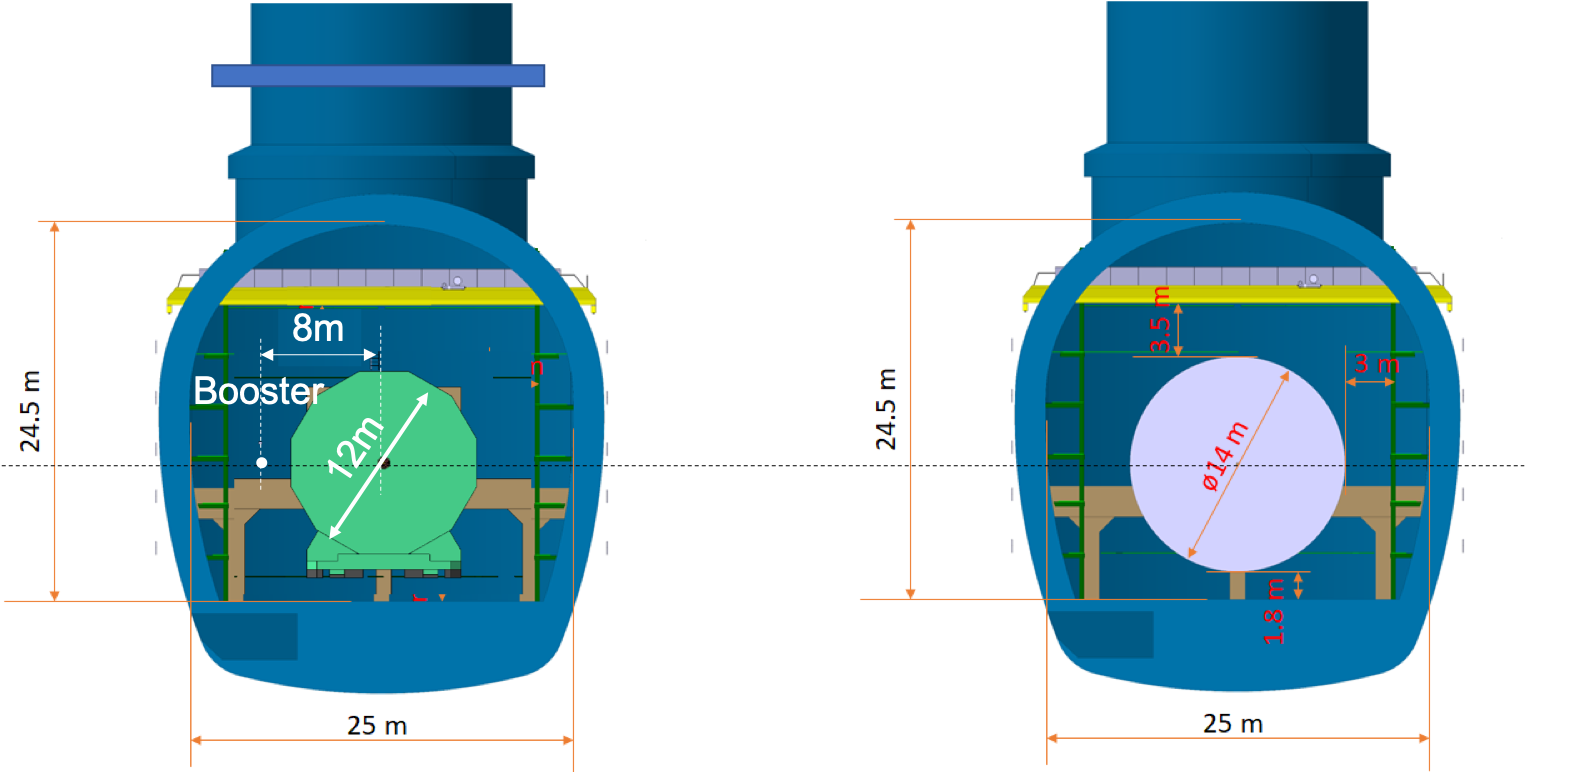
\includegraphics[width=0.9\textwidth]{Caverns/Figs/large_small_cavern.png}
\caption{An FCC-ee detector (left) and the FCC-hh reference detector (right) 
in a small cavern of 24.5\,m $\times$ 25\,m cross section.}
\label{small_cavern}
\end{figure}

In FCC-hh, the longitudinal extent of the detector is limited by the machine elements and the related shielding. 
The last magnetic elements in the final focusing magnets of FCC-hh are at $\ell^* = 40$\,m from the interaction point. 
In order to shield these magnets from the collision debris originating from the interaction point, 
the so-called `TAS absorbers' are placed at a distance of around 35\,m. 
The absorption of these high energy hadrons produces a significant amount of neutrons that `diffuse' out of this absorber, 
as can be appreciated in Fig.~\ref{radiation}. 
The concrete cavern wall at $z = 33$\,m stops these neutrons from entering the cavern, 
defining the maximum possible cavern length to be 66\,m.
Altogether, these basic considerations converge to a cavern size of L66\,m $\times$ W35\,m $\times$ H35\,m for the FCC-hh reference detector.

\begin{figure}[ht]
\centering
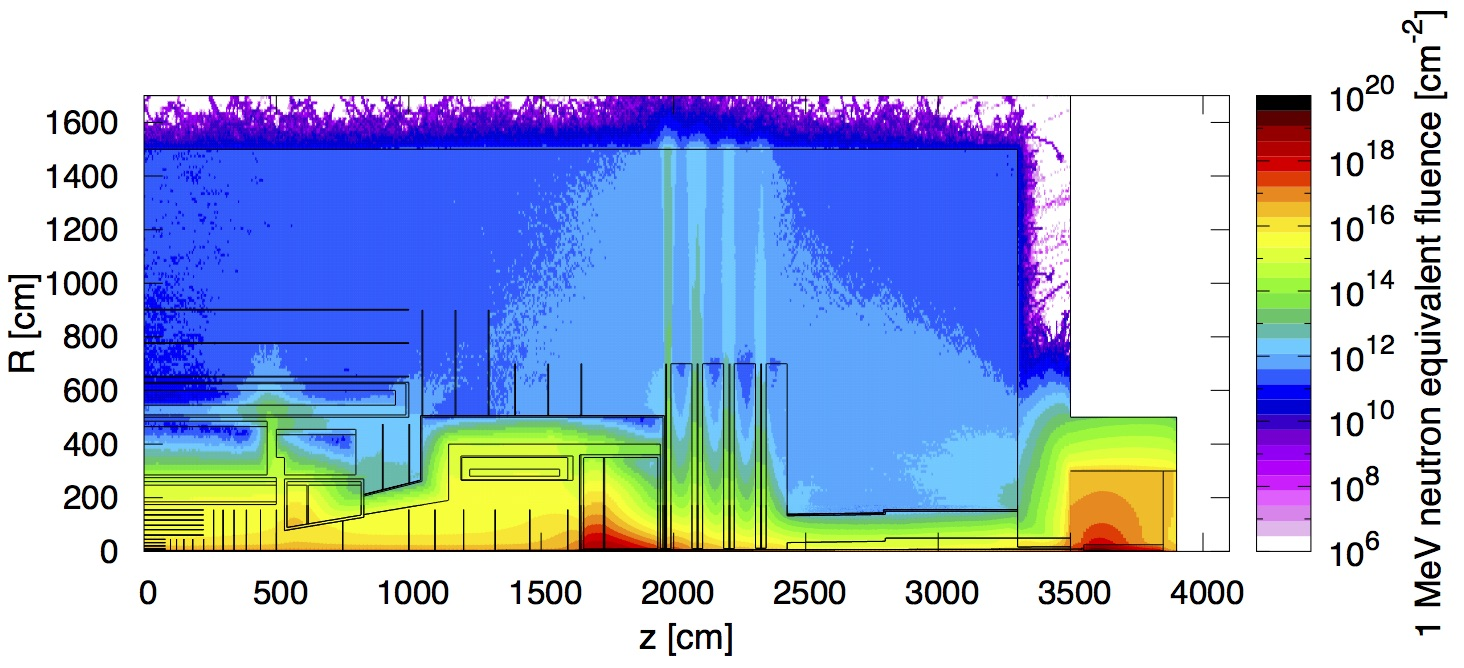
\includegraphics[width=0.95\textwidth]{Caverns/Figs/1MeVeqF_newLstar.jpg}
\caption{Radiation load for the FCC-hh detector and the final focusing magnets in the machine tunnel.}
\label{radiation}
\end{figure}

\subsection{FCC cavern infrastructure}

The FCC-hh cavern infrastructure is shown in Fig.~\ref{infrastructure}. 
Since the service cavern is at a distance of around 50\,m from the detector cavern and between 60 and 70\,m away from the beamline, 
the stray field therein is below 5\,mT (Fig.~\ref{bfield}) and standard equipment can be placed at this location.
Besides, the radiation shielding provided by this distance suffices to allow permanent access to the service cavern. 
A main shaft of 18\,m diameter gives access from the surface to the experiment cavern. 
It houses only some ventilation pipes but no other services or elevators, and is only foreseen for the transport of equipment. 
The personnel access and the detector services are housed in the service shaft, which connects to the service cavern. 
Three connection tunnels, represented in Fig.~\ref{infrastructure}, connect the service and experiment caverns: 
a central one, of 10\,m diameter, for services, and two others, of 5.5\,m diameter, placed on each of the two ends of the detector. 
They are complemented by two evacuation tunnels, also represented in the figure.

\begin{figure}[h]
\centering
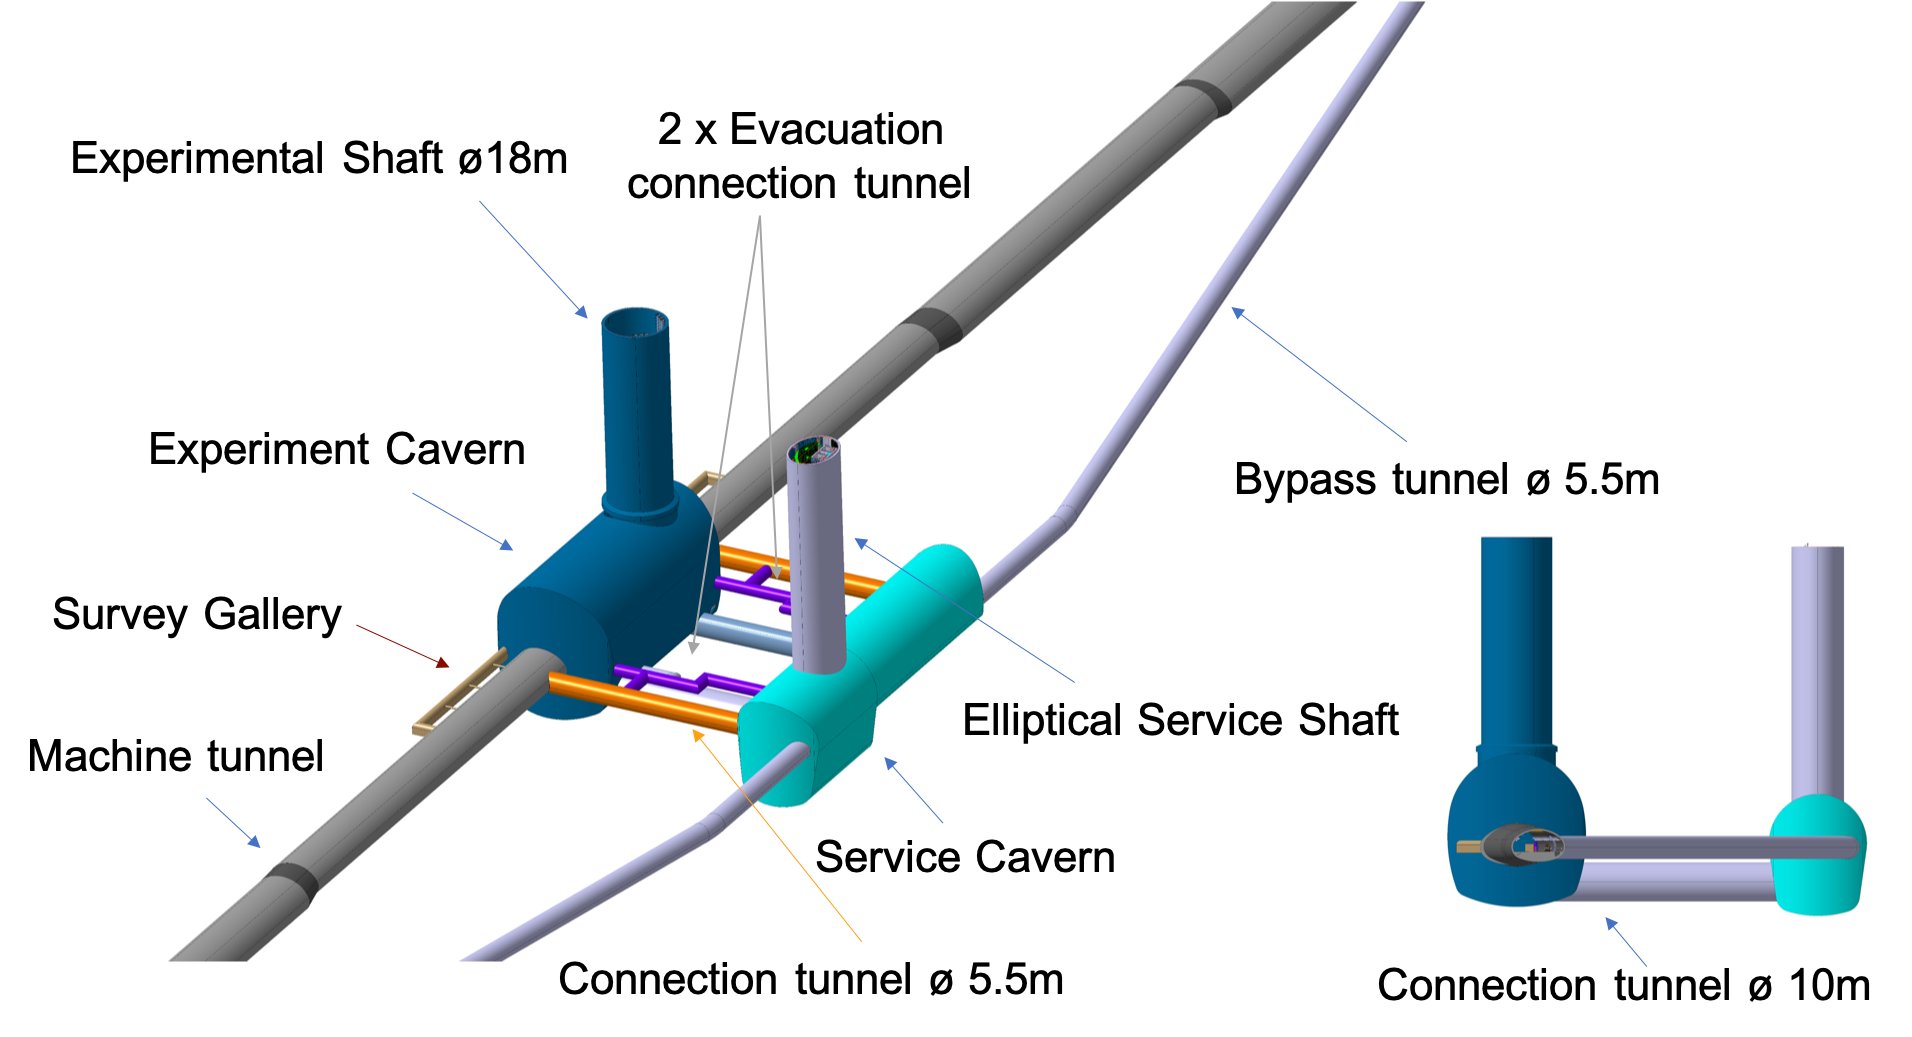
\includegraphics[width=0.9\textwidth]{Caverns/Figs/fcc_cavern_infrastructure.png}
\caption{FCC-hh cavern infrastructure.}
\label{infrastructure}
\end{figure}

The principal dimensions of the FCC cavern infrastructure are summarised in Table~\ref{t1}.

\begin{table}[ht]
\caption{Requirements and key numbers for the FCC-ee and FCC-hh detectors.}
\label{t1}
\centering
  \begin{tabular}{l c}
  \hline
    Item &  \\
    \hline
     Size of large caverns & L66\,m W35\,m H35\,m  \\
     Shaft diameter of large caverns & 18\,m \\
     Size of small caverns & L66\,m W25\,m H24.5\,m  \\
     Shaft diameter of small caverns & 14\,m \\
     \hline
     FCC-hh reference detector diameter without yoke & 20\,m \\
     FCC-hh reference detector diameter with yoke & 22\,m \\
     Stray field at cavern wall ($R = 17.5$\,m) & 100\,mT \\
     Distance for stray field $<5$\,mT & 55\,m \\
     \hline
     FCC-ee detector diameter & 12--14\,m \\
    \hline
  \end{tabular}
\end{table}
